\chapter{气孔导度和光合作用}
%\addcontentsline{toc}{chapter}{气孔导度和光合作用}

%\begin{气孔导度和光合作用}

\section{气孔导度}\label{气孔导度}
气孔导度是地表湍流方案水通量计算中的一个重要的参数 (见章节4.3),制约着植被蒸腾。同时,
气孔导度与光合作用相耦合,在植物生理模块中,CoLM分别计算阳叶和阴叶的气孔导度 ($g_{s,sun}$和$g_{s,sha}$),控制着植被与大气之间的碳水交换。


CoLM的气孔导度计算仍沿用Ball-Berry模型。Ball-Berry模型根据叶片净光合作用速率 
($A_n$,单位: $\rm mol\ CO_2\ m^{-2}s^{-1}$)、叶表水汽压 ($e_s$,单位: Pa)、叶表二氧化碳分压 ($c_s$,单位: Pa) 
基于气孔导度的观测回归经验关系,计算气孔导度 ($g_s$, 单位: $\rm mol\ CO_2\ m^{-2}s^{-1}$): 
\begin{equation}\label{rs_a1}
\frac{1}{r_{s}}=g_{s}=m \frac{A_{n}}{c_{s}} \frac{e_{s}}{e_{i}} p_{s}+b
\end{equation}
$r_s$代表叶片气孔阻抗,单位: $\rm s\ m^{-1}$;$m$是无量纲经验参数;$b$是最小气孔导度,
单位: $\rm mol\ CO_2\ m^{-2}s^{-1}$,$m$和$b$是观测拟合的经验系数;$e_i$是饱和水蒸气压,
是气温的函数,单位: Pa;$p_s$是大气压强,单位: Pa。
\section{植物的光合作用}\label{植物的光合作用}
C3植物的光合作用模拟是基于Farquhar光合作用模型 \citep{farquhar1980biochemical} ,
C4植物则是基于\citet{collatz1992} 的光合作用改进模型。
光合作用受到三方面的限制,即RuBP羧化酶的限制,RuBP再生速率的限制和羧化产物速率的限制,相应的受限羧化速率分别为:$A_{c}$, $A_{j}$, $A_{e}$。叶片净光合作用速率 ($A_{n}$) 等于受限光合羧化速率减去叶呼吸速率 ($R_d$):
\begin{equation}\label{An1}
A_{n}=\min \left(A_{c}, A_{j}, A_{e}\right)-R_{d}
\end{equation}


RuBP羧化酶限制主要指当羧化酶浓度不足时,光合作用最大羧化速率$V_{c \max }$受限。RuBP羧化酶限制下的最大羧化率 ($A_c$) 可表达为$V_{c \max }$的函数,其中C3植物羧化速率受到胞间CO$_2$分压$c_i$的调节,并表达为Michaelis-Menten函数:
\begin{equation}\label{A_C1}
A_{c}=\left\{\begin{array}{ll}\frac{V_{c \max }\left(c_{i}-\Gamma\right)}{c_{i}+K_{c}\left(1+\frac{o_{i}}{K_{o}}\right)}
     & { for\ } \mathrm{ C3\ } \mathrm{ plants } \\ V_{c \max } & { for\ } \mathrm{ C4\ } \mathrm{ plants }\end{array}\right.
\end{equation}
其中,$\Gamma$是CO$_2$补偿点,$K_c$和$K_o$分别是对于CO$_2$和O$_2$的Michaelis-Menten常数(Pa),$o_i$是氧气分压(Pa)。\\
C3植物:\\
\begin{equation}\label{V_cmax_a}
V_{c \max }\left(T_{{leaf }}\right)=V_{c \max 25} \cdot \frac{2.1^{\frac{T_{{leaf }}-T_{o p}}{10}}}{1+e^{s_{1}\left(T_{{leaf }}-T_{{high }}\right)}} \cdot \beta
\end{equation}
$C_4$植物:\\
\begin{equation}\label{V_cmax_b}
V_{c \max }\left(T_{{leaf }}\right)=V_{c \max 25} \cdot \frac{2.1^{\frac{T_{{leaf }}-T_{o p}}{10}}}{\left(1+e^{s_{2}\left(T_{{low }}
 - T_{{leaf }}\right)}\right)\left(1+e^{s_{1}\left(T_{{leaf }}-T_{h i g h}\right)}\right)} \cdot \beta
\end{equation}
$V_{c \max 25}$是25$\textcelsius$下的最大羧化速率,单位: $\mathrm{mol\ m^{-2}s^{-1}}$;$T_{op}$是参考温度298 K;$s_1$和$s_2$分别为高温和低温的温度敏感性参数;$T_{low}$和$T_{high}$分别为羧化速率的低温和高温响应参数,
取值根据植被类型而变化,范围分别为: 278K$\sim$288K,303$\sim$313K;$T_{leaf}$是叶片温度,通过对叶片能量平衡方程进行牛顿迭代方法而求解得到,详见章节\ref{植被叶片温度计算},$\beta$是植物水分胁迫因子,取值范围0$\sim$1,详见章节 \ref{气孔导度的水分胁迫}。

当光照不足时,RuBP再生速率下降,成为制约光合作用开尔文循环的最主要因素。因此,RuBP再生速率限制下的羧化速率 ($A_j$) 可表达为有效光合辐射 ($PAR$) 的函数:
\begin{equation}\label{A_J1}
A_{J}=\left\{\begin{array}{ll}\frac{J_x\left(PAR\right)\left(c_{i}-\Gamma\right)}{4c_{i}+8\Gamma}
     & { for\ } \mathrm{ C3\ } \mathrm{ plants } \\ \alpha\left(4.6\phi\right) & { for\ } \mathrm{ C4\ } \mathrm{ plants }\end{array}\right.
\end{equation}

$J_x$是有效光合辐射(PAR)的函数,并受叶片温度 ($T_{leaf}$) 的调节:
\begin{equation}
J_{x}\left(T_{{leaf }}\right)=\min \left(\alpha\left(4.6 \times 10^{-6} \cdot PAR\right), J_{\max 25}
 \cdot e^{\frac{37000\left(T_{{leaf }}-T_{o p}\right)}{T_{o p} \cdot T_{{leaf }} \cdot R} \cdot \frac{1+e^{\frac{710 \cdot T_{o p}-220000}
 {R \cdot T_{o p}}}}{\frac{710 \cdot T_{{leaf }}-220000}{R \cdot T_{{leaf }}}}}\right) \cdot \beta
\end{equation}
其中$\alpha$是量子效率 (0.05 mol CO$_2$ $\rm mol^{-1}$ photon);$PAR$是有效光合辐射,单位: $\rm W m^{-2}$,详细计算见章节~\ref{短波吸收辐射通量};
$4.6 \times 10^{-6}$代表单位从$\rm W m^{-2}$转换到$\mathrm{mol\ photon\ m^{-2}}$的转换系数;
$J_{\max 25}$是25 \textcelsius 下的最大电子传输速率,单位: $\mathrm{mol\ m^{-2}s^{-1}}$,$J_{\max 25}=1.97 \cdot V_{c \max 25}$; 
$R$是通用气体常数,$R=8.314467591$ $\mathrm{mol\ m^{-2}s^{-1}}$。

羧化产物速率限制下的羧化速率 ($A_e$) 是25 \textcelsius 最大羧化速率常数 ($V_{c \max}$) 的函数,并且受到叶温和水分胁迫因子的调控:、\\
C3植物:\\
\begin{equation}\label{A_e_a}
A_e=\frac{V_{c \max 25}}{2} \cdot \frac{1.8^{\frac{T_{{leaf }}-T_{o p}}{10}}}{1+e^{s_{2}\left(T_{{leaf }}-T_{{low }}\right)}} \cdot \beta
\end{equation}
$C_4$植物:\\
\begin{equation}\label{A_e_b}
A_e=\frac{V_{c \max 25}}{5} \cdot 1.8^{\frac{T_{{leaf }}-298.16}{10}} \cdot \beta
\end{equation}
三方面限制下的羧化速率均共用同一套温度响应常数 ($T_{op}$,$T_{low}$和$T_{high}$)


呼吸速率对温度的响应曲线可表示为$V_{c \max25}$的函数:
\begin{equation}\label{R_d1}
R_{d}=r_{{base }} \cdot V_{cmax 25} \cdot \frac{2.0^{\frac{T_{leaf}-T_{op}}{10}}}{1+e^{s_3 \cdot\left(T_{leaf}-T_{d m}\right)}} \cdot \beta
\end{equation}
其中$T_{dm}$是叶呼吸的高温抑制温度常数,单位 K。



在求解最小值的计算中,我们将三值最小问题的求解拆分为两个二值最小问题的求解:
\begin{equation}\label{min_Ac_Aj_Ae}
\min \left(A_{c}, A_{j}, A_{e}\right)=\min \left(\min \left(A_{c}, A_{j}\right), A_{e}\right)
\end{equation}
引入形状参数$\theta$,构造一元二次方程,将求解最小值问题转换成求一元二次方程较小根的问题,以此避免最小值随环境变化引起的结果突变 \citep{collatz1991,collatz1992}:
\begin{equation}\label{theta_cj}
\theta_{c j} \cdot A_{i1}^{2}-\left(A_{c}+A_{j}\right) A_{i1}+A_{c} A_{j}=0
\end{equation}
\begin{equation}\label{theta_cje}
\theta_{c j e} \cdot A_{i2}^{2}-\left(A_{i1}+A_{e}\right) A_{i2}+A_{i1} A_{e}=0
\end{equation}
其中形状参数$\theta_{cj}=0.877$,$\theta_{cje}=0.95$。$A_{i1}$为方程(\ref{theta_cj})的较小根,代表$A_c$和$A_j$的最小值。$A_{i2}$为方程(\ref{theta_cje})的较小根,代表$A_{i1}$和$A_e$的最小值。


另外,气孔导度方程~\eqref{rs_a1} 仍然存在胞间CO$_2$分压$c_i$ (Pa),叶表CO$_2$分压$c_s$ (Pa),叶表水汽分压$e_s$ (Pa)等未知变量,
耦合光合作用模型对气孔导度方程求解,需要包括气孔内外的扩散方程:
\begin{equation}\label{A_n2}
A_{n}=\left(c_{a}-c_{s}\right) /\left(\frac{1.37}{g_{b}} p_{s}\right)=\left(c_{s}-c_{i}\right) /\left(\frac{1.6}{g_{s}} p_{s}\right)
\end{equation}
\begin{equation}\label{ea_ei}
\left(e_{a}-e_{i}\right) /\left(\frac{1}{g_{b}}+\frac{1}{g_{s}}\right)=\left(e_{s}-e_{i}\right) / \frac{1}{g_{s}}
\end{equation}
$c_a$是冠层大气$\rm CO_2$分压,单位: Pa;$g_b$是叶片边界层导度,单位: $\mathrm{mol\ m^{-2}s^{-1}}$;$e_a$是冠层大气水汽分压,单位: Pa,$e_i$是胞间水汽分压,单位: Pa。

由方程~\eqref{A_n2} 可知:
\begin{equation}\label{cs_a1}
c_{s}=c_{a}-\frac{1.37 A_{n}}{g_{b}} p_{s}
\end{equation}
由方程~\eqref{ea_ei} 可知:
\begin{equation}\label{e_s1}
e_{s}=\left(\frac{e_{a}}{g_{s}}+\frac{e_{i}}{g_{b}}\right) /\left(\frac{1}{g_{b}}+\frac{1}{g_{s}}\right)
\end{equation}
将方程~\eqref{e_s1} 代入方程~\ref{rs_a1} 中,得到关于$g_s$的一元二次方程:
\begin{equation}\label{ei_cs}
\frac{e_{i} c_{s}}{m A_{n} p_{s}} g_{s}^{2}+\left(g_{b} \frac{e_{i} c_{s}}{m A_{n} p_{s}}-e_{i}-b \frac{e_{i} c_{s}}{m A_{n} p_{s}}\right) g_{s}
-\left(e_{a} g_{b}+b g_{b} \frac{e_{i} c_{s}}{m A_{n} p_{s}}\right)=0
\end{equation}
气孔导度 ($g_s$) 的解即为一元二次方程的正根,其中叶片表层$\mathrm{CO_2}$分压 ($c_s$) 由方程~\eqref{cs_a1} 得出,$A_n$由光合作用模块公式~\eqref{An1} 得出,
但仍然包含未知变量胞间 $\mathrm{CO_2}$ 分压 ($c_i$),完整求解光合气孔模式还需根据~\eqref{A_n2} 得出:
\begin{equation}\label{ci_1}
c_{i}=c_{s}-\frac{1.6 A_{n} p_{s}}{g_{s}}
\end{equation}
联立~\eqref{An1}, \eqref{cs_a1}, \eqref{ei_cs} 和 \eqref{ci_1} 可以求解 $g_s$,$c_i$,$c_s$ 和 $A_n$。
通过牛顿迭代数值解法,对胞间$\mathrm{CO_2}$分压 $c_i$ 求解,从而求解所有未知量。

{
\begin{figure}[]
\centering
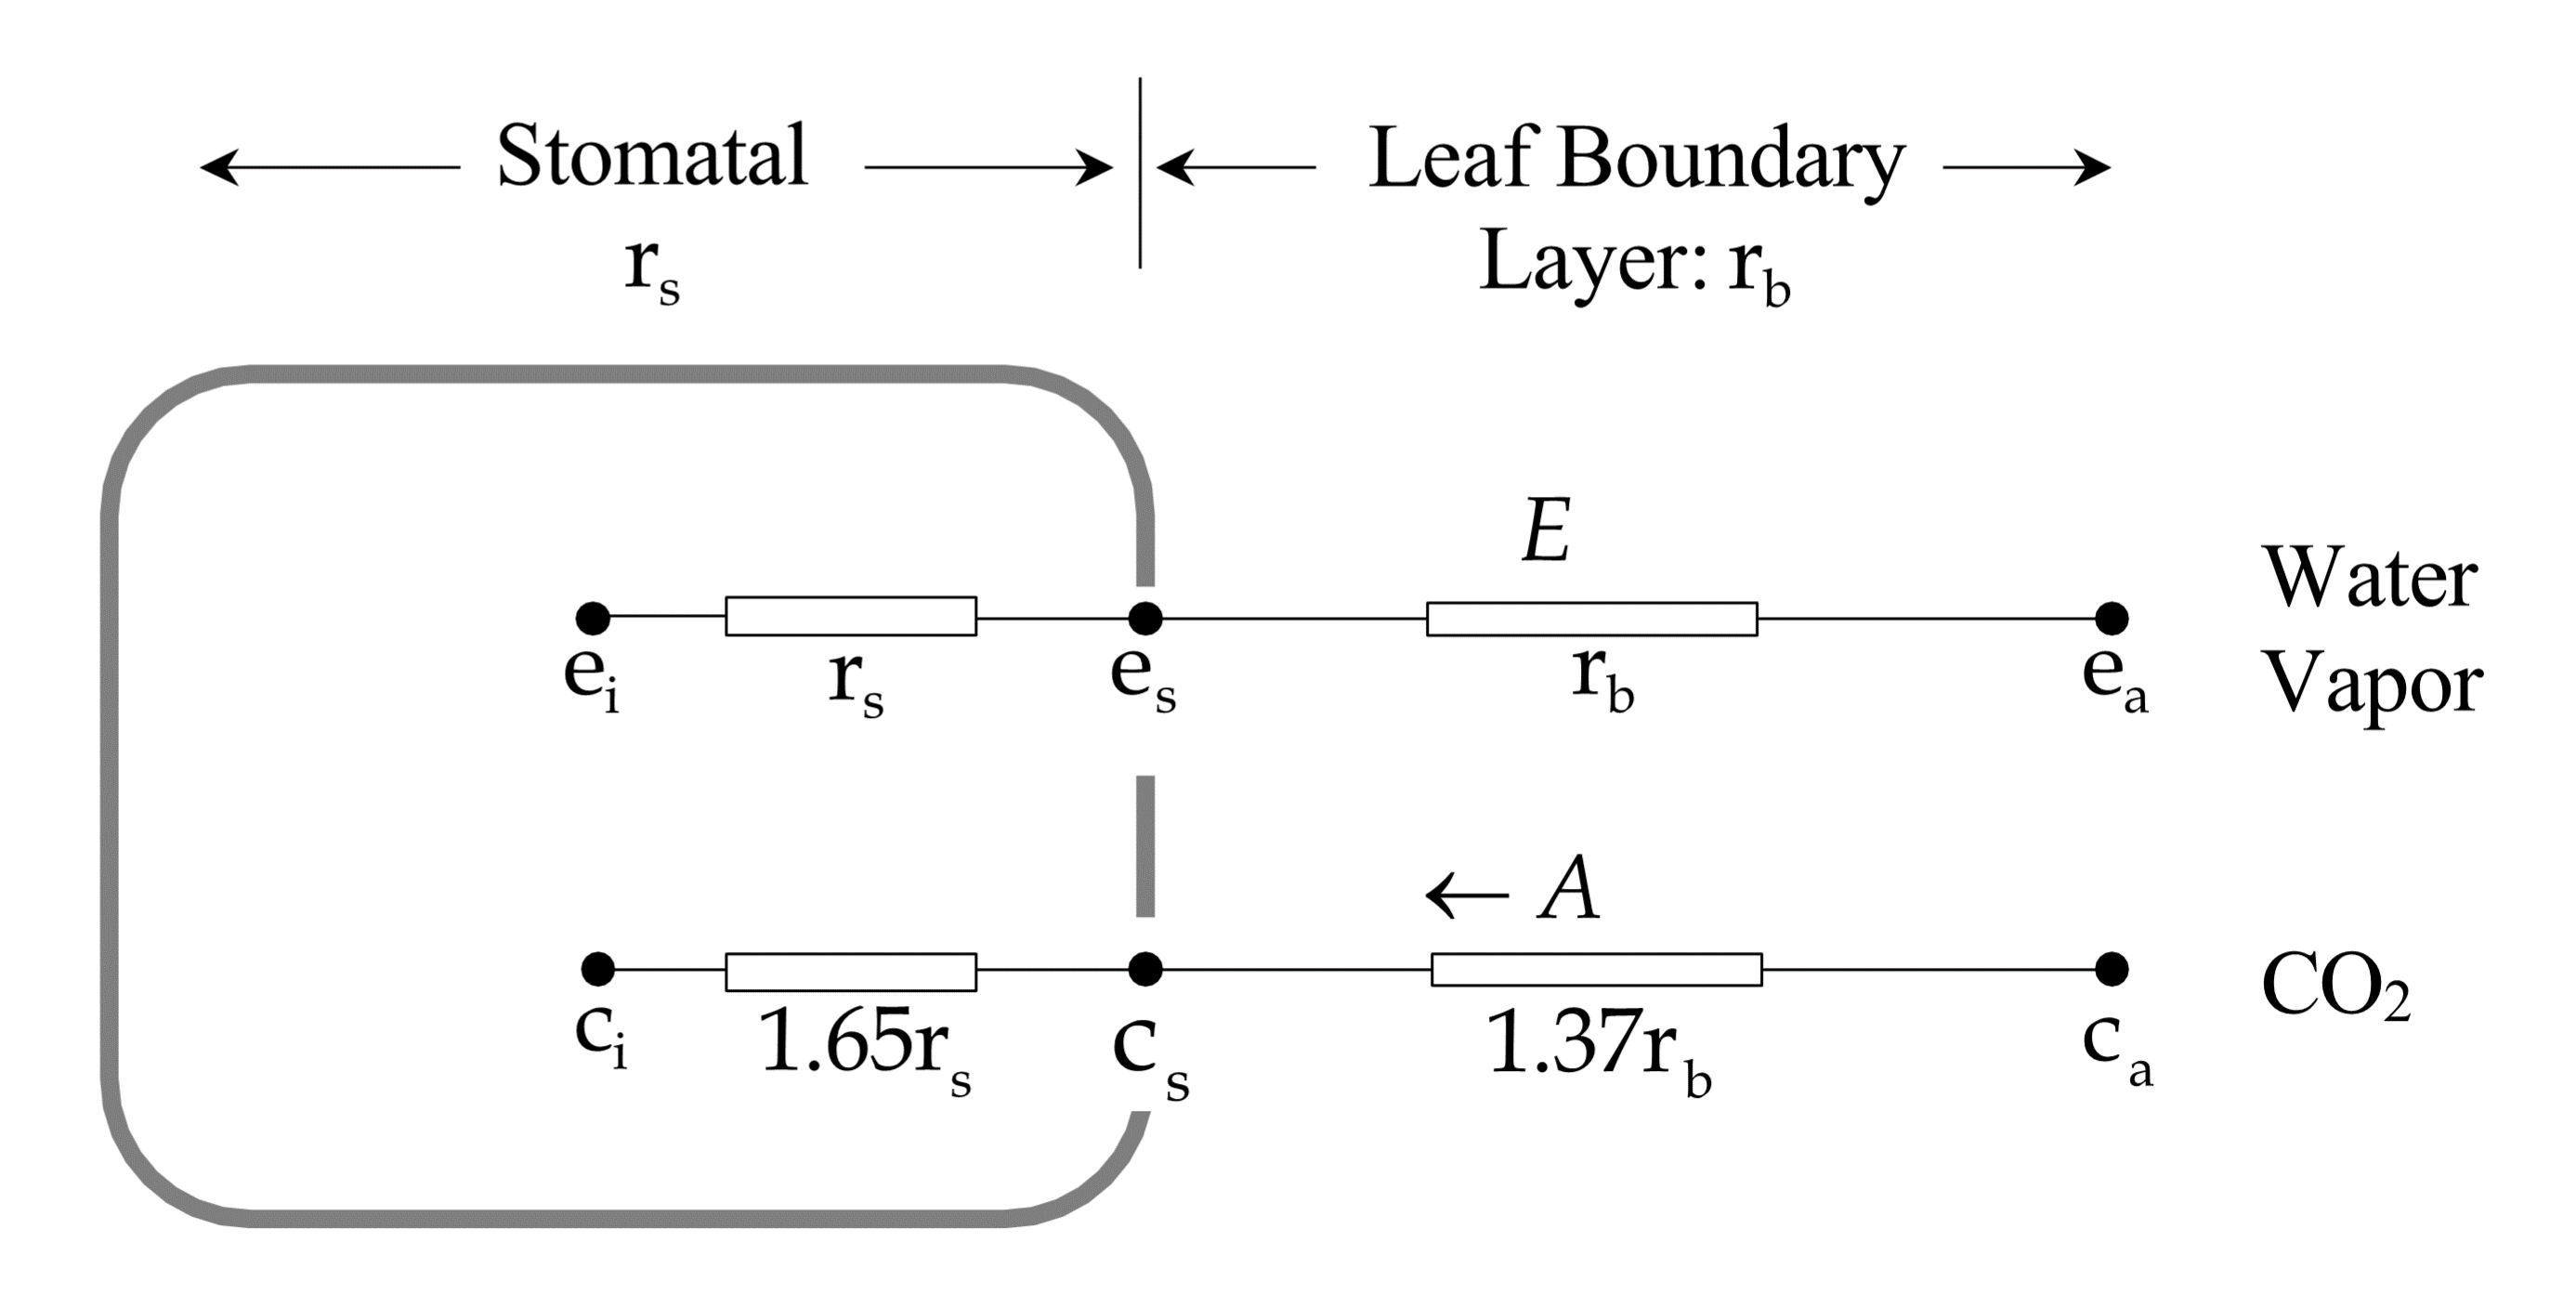
\includegraphics{Figures/气孔导度和光合作用/叶片气孔光合作用导度模型示意图.png}
\caption{叶片气孔光合作用导度模型示意图。}
\label{fig:叶片气孔光合作用导度模型示意图}
\end{figure}
}
